\documentclass[a4paper, 12pt]{article}
\usepackage[utf8]{inputenc}
\usepackage[warn]{mathtext}
\usepackage[russian]{babel}
\usepackage[T2]{fontenc}
\usepackage[warn]{mathtext}
\usepackage[justification=centering]{caption}

\usepackage{graphicx}
\graphicspath{ {images/} }
\usepackage{tikz}
\usepackage{pgfplots}

\usepackage{amsmath}
\usepackage{floatflt}
\usepackage[left=20mm, top=20mm, right=20mm, bottom=20mm, footskip=10mm]{geometry}

\usepackage{multicol}
\usepackage{multirow}
\setlength{\columnsep}{2cm}

\usepackage{multicol}
\setlength{\columnsep}{2cm}
\usepackage{hyperref}
\usepackage{wrapfig}

\begin{document}
	
\begin{titlepage}
	\centering
	\vspace{5cm}
	{\scshape\LARGE Московский физико-технический институт \par}
	\vspace{4cm}
	{\scshape\Large Лабораторная работа 5.1.1 \par}
	\vspace{1cm}
	{\huge\bfseries Фотоэффект \par}
	\vspace{1cm}
	\vfill
\begin{flushright}
	{\large выполнил студент 924 группы ФОПФ}\par
	\vspace{0.3cm}
	{\LARGE Панферов Андрей}
\end{flushright}
	

	\vfill

% Bottom of the page
	Долгопрудный, 2021 г.
\end{titlepage}

    \paragraph*{Цель работы:} Исследовать зависимость фототока от величины задерживающего потенциала и частоты падающего излучения, что позволяет вычислить величину постоянной Планка.

    \section*{Теоретическая часть}

    Фотоэффект --- явление испускания электронов фотокатодом, облучаемым светом,  Это явление хорошо объясняется фотонной теорией света. Взаимодействие монохроматического света с веществом можно описывать
	как взаимодействие с веществом частиц, называемых фотонами, которые обладают энергией $ \hbar \omega $ и импульсом $ \hbar\omega/c $. При столкновении фотона с электроном фотокатода энергия отона полностью передается электрону, и фотон прекращает свое существование. Энергетический баланс этого взаимодействия для вылетающих электронов
	описывается уравнением
	
	\begin{equation}\label{energy balance}
	\hbar \omega = E_{max} + W
	\end{equation}
	
	\begin{wrapfigure}{l}{0.4\linewidth}
		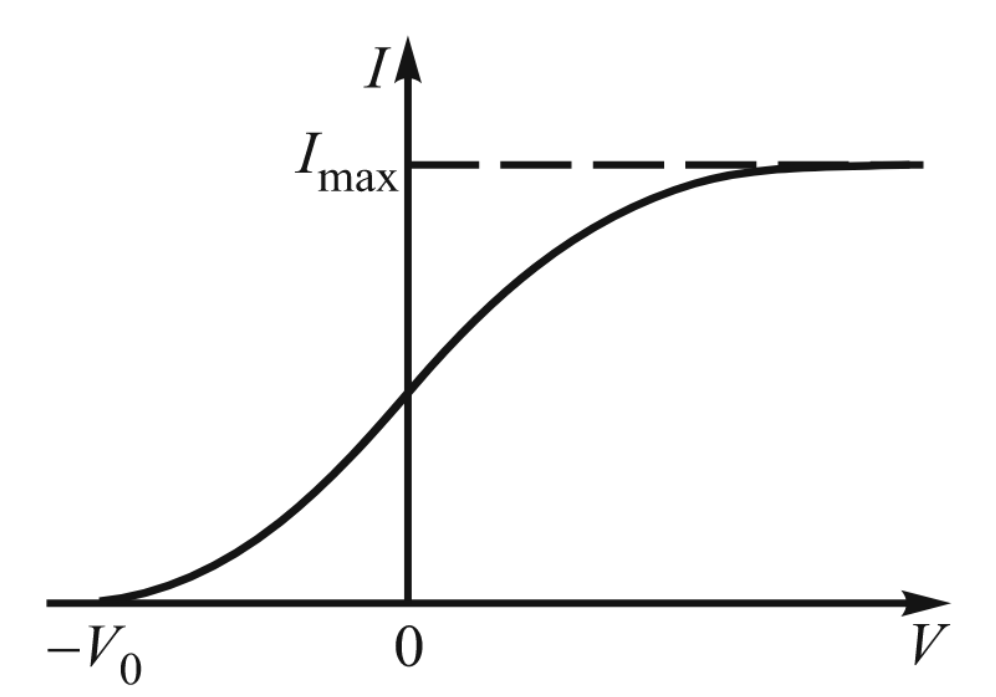
\includegraphics[width=\linewidth]{I_V.png}
		\caption{Зависимость фототока от напряжения на аноде фотоэлемента}
		\label{ris I(V)}
	\end{wrapfigure}
	
	Здесь $ E_{max} $ ---  максимальная кинетическая энергия электрона после выхода из фотокатода, $ W $ --- работа выхода электрона из катода. Реально энергетический спектр вылетевших из фотокатода электронов непрерывен --- он простирается от нуля до $ E_{max} $. 
	
	Для измерения энергии вылетевших фотоэлектронов вблизи фотокатода
	обычно располагается второй электрод
	(анод), на который подается задерживающий ($ V < 0 $) или ускоряющий ($ V >
	0 $) потенциал. При достаточно больших
	ускоряющих напряжениях фототок достигает насыщения (рис. \ref{ris I(V)}): все испущенные электроны попадают на анод.
	
	При задерживающих потенциалах на анод попадают лишь электроны,
	обладающие достаточно большой кинетической энергией, в то время
	как медленно движущиеся электроны заворачиваются полем и возвращаются на катод. При некотором значении $ V = -V_0 $ (потенциал запирания) даже наиболее быстрые фотоэлектроны не могут достичь
	анода.
	Максимальная кинетическая энергия $ E_{max} $ электронов связана с
	запирающим потенциалом $ V_0 $ очевидным соотношением $ E_{max} = eV_0 $. Тогда \eqref{energy balance} примет вид, называемый уравнением Эйнштейна:
	
	\begin{equation}\label{Einsteain}
	eV_0 = \hbar\omega - W 
	\end{equation}
	
	Чтобы определить величину запирающего
	напряжения, нам надо правильно экстраполировать получаемую токовую зависимость к нулю, т. е. определить, какова функциональная
	зависимость $ I(V) $. Расчет для простейшей геометрии --- плоский катод, освещаемый светом, и параллельный ему анод --- приводит к зависимости
	
	\begin{equation}\label{sqrt I = V}
	\sqrt{I} \propto V_0 - V
	\end{equation}
	
	т. е. корень квадратный из фототока линейно
	зависит от запирающего напряжения. Эта зависимость хорошо описывает экспериментальные данные.
	
	В работе изучается зависимость фототока из фотоэлемента от величины задерживающего потенциала $ V $ для различных частот света $ \omega $, лежащих в видимой области спектра. С целью экспериментальной
	проверки уравнения Эйнштейна определяются потенциалы запирания
	$ V_0 $ при разных частотах света и строится зависимость $ V_0(\omega) $, которая, как это следует из \eqref{Einsteain}, должна иметь вид
	
	\begin{equation}\label{V(w)}
	V_0 (\omega) = \dfrac{\hbar\omega - W}{e}
	\end{equation}
	
		\begin{wrapfigure}{r}{0.4\linewidth}
		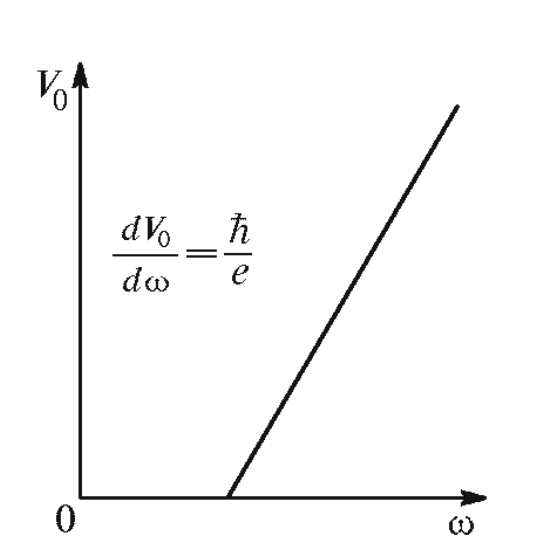
\includegraphics[width=\linewidth]{V_w.png}
		\caption{Зависимость запирающего потенциала
			от частоты света}
		\label{ris V(w)}
	\end{wrapfigure}
	
	Потенциал запирания $ V_0 $ для любого катода линейно зависит от
	частоты света $ \omega $. По наклону прямой на графике $ V_0(\omega) $ (рис. \ref{ris V(w)}) можно определить постоянную Планка:
	
	\begin{equation}\label{dV/dw}
	\dfrac{dV_0}{d\omega} = \dfrac{\hbar}{e}
	\end{equation}
	
	Как показывает формула \eqref{dV/dw}, угол наклона прямой $ V_0(\omega) $ не зависит от рода вещества, из которого изготовлен фотокатод. От рода вещества, однако, зависит величина фототока, работа выхода $ W $ и форма кривой $ I(V) $ (рис. \ref{ris I(V)}). Все это определяет выбор пригодных для
	опыта катодов.


    \section*{Выполнение работы}
	
	Сначала выполним градуировку монохроматора. Проведем серию измерений для линий спектра неона, снимая зависимость длины волны света от параметра $ \theta $ барабана монохроматора. Результаты занесем в Таблицу \ref{table:grad} и построим График \ref{graph:grad} зависимости, профитировав функцию $ \lambda (\theta) $ многочленом второй степени в силу нелинейности. 
	
	\begin{figure}[h]
		\begin{minipage}{0.4\textwidth}
		        \centering
		        \begin{tikzpicture}
                    \centering
                    \label{graph:grad}
                    \begin{axis}[
                        	axis lines = middle,
                        	xlabel = {$\theta$, $ ^\circ $},
                            ylabel = {$ \lambda, \;\mathring{A} $},
                        	ylabel style={red, scale=1},
                            xlabel style={red, scale=1},
                            title style={align=left}, title={Зависимость длины волны от угла},
                        	table/col sep=comma,
                            error bars/y dir=both,
                            error bars/y fixed=2,
                        ]
                	    \addplot +[black, only marks] table[x=THETA, y=LAMBDA]{calibration.txt};
                	\end{axis}
                \end{tikzpicture}
		\end{minipage}
		\hfill
		\begin{minipage}{0.4\textwidth}
		    \centering
                \captionof{table}{Градуировка монохроматора}
                \label{table:grad}
                \begin{tabular}{|cc|}
                \hline
                \multicolumn{1}{|c|}{$\theta$, $ ^\circ $} & $ \lambda, \;\mathring{A} $ \\ \hline
                2296                                       & 5852                        \\
                2342                                       & 5945                        \\
                2412                                       & 6096                        \\
                2434                                       & 6143                        \\
                2534                                       & 6402                        \\
                2574                                       & 6507                        \\
                2644                                       & 6717                        \\
                2038                                       & 5401                        \\ \hline
                \end{tabular}  
		\end{minipage}
    \end{figure}

\begin{table}[h]
    \centering
    \caption{Фототок}
    \label{table:main}
    \begin{tabular}{|cc|cc|cc|}
    \hline
    \multicolumn{2}{|l|}{\begin{tabular}[c]{@{}l@{}}$\lambda = 5401\mathring{A}$\\ $\theta = 2038^\circ$\end{tabular}} & \multicolumn{2}{l|}{\begin{tabular}[c]{@{}l@{}}$\lambda = 5860\mathring{A}$\\ $\theta = 2300^\circ$\end{tabular}} & \multicolumn{2}{l|}{\begin{tabular}[c]{@{}l@{}}$\lambda = 6717\mathring{A}$\\ $\theta = 2644^\circ$\end{tabular}} \\ \hline
    $V_I$, V                                                 & $V$, V                                                & $V_I$, V                                                & $V$, V                                               & $V_I$, V                                                & $V$, V                                                \\ \hline
    0.51                                                      & 0.726                                                  & 0.54                                                     & 0.726                                                 & 0.56                                                     & 0.726                                                  \\ \hline
    0.26                                                      & -0.107                                                 & 0.25                                                     & -0.117                                                & 0.30                                                     & 0.047                                                  \\ \hline
    0.30                                                      & -0.043                                                 & 0.30                                                     & -0.070                                                & 0.35                                                     & 0.081                                                  \\ \hline
    0.35                                                      & 0.034                                                  & 0.35                                                     & -0.020                                                & 0.40                                                     & 0.125                                                  \\ \hline
    0.40                                                      & 0.136                                                  & 0.40                                                     & 0.050                                                 & 0.45                                                     & 0.200                                                  \\ \hline
    0.45                                                      & 0.300                                                  & 0.45                                                     & 0.164                                                 & 0.50                                                     & 0.350                                                  \\ \hline
                                                              &                                                        & 0.50                                                     & 0.395                                                 &                                                          &                                                        \\ \hline
    \end{tabular}
\end{table}
	
	Теперь проведем 3 серии измерений зависимости фототока от напряжения для разных длин волн падающего света, изменяя на монохроматоре параметр $ \theta $ и переводя его в длину волны с помощью градуировки. Ток приведен в безразмерных единицах в силу работы установки. 
	
	Результаты измерений занесем в Таблицу \ref{table:main}. Вблизи потенциала запирания, искомая зависимость описывается формулой \eqref{sqrt I = V}. Согласно этой формуле \eqref{sqrt I = V}, построим График \ref{fig:3freq} зависимости в координатах $ \sqrt{I} (V) $ и аппроксимируем линейные участки прямой. Экстраполируя прямую к нулю, получим значения потенциала запирания для каждой серии измерения (длины волны). Результаты сведем в Таблицу \ref{table:3freq}. 


\begin{figure}[h]
    \centering
    \label{fig:3freq}
    \begin{tikzpicture}
        \centering
        \label{graph:grad}
        \begin{axis}[
            	axis lines = middle,
            	xlabel = {$V$, V},
                ylabel = {$\sqrt{V_I},\:\sqrt{V}$},
            	ylabel style={red, scale=1},
                xlabel style={red, scale=1},
                title style={align=left}, title={Зависимость фототока от напряжения},
                width=15cm, height=10cm,
            ]
            \addplot +[red, only marks,
                table/col sep=comma,
                error bars/y dir=both,
                error bars/y fixed=0.01,
                error bars/x dir=both,
                error bars/x fixed=0.01,] table[x=V1, y=SQRT_I1]{3freq.txt};
            \addplot[color=red, domain=-0.12:0.2]{0.575 + 0.72 * x};
            
            \addplot +[green, only marks,
                table/col sep=comma,
                error bars/y dir=both,
                error bars/y fixed=0.01,
                error bars/x dir=both,
                error bars/x fixed=0.01,] table[x=V2, y=SQRT_I2]{3freq.txt};
            \addplot[color=green, domain=-0.12:0.2]{0.61 + 0.92 * x};
             
            \addplot +[blue, only marks,
                table/col sep=comma,
                error bars/y dir=both,
                error bars/y fixed=0.01,
                error bars/x dir=both,
                error bars/x fixed=0.01,] table[x=V3, y=SQRT_I3]{3freq.txt};
            \addplot[color=blue, domain=0:0.2]{0.5 + x};
            
            \legend{$\lambda = 5401\mathring{A}$,
                    linear,
                    $\lambda = 5860\mathring{A}$,
                    linear,
                    $\lambda = 6717\mathring{A}$,
                    linear,}
        \end{axis}
    \end{tikzpicture}
\end{figure}

\begin{table}[h]
    \centering
    \label{table:3freq}
    \caption{Зависимость запирающего напряжения от частоты}
    \begin{tabular}{|l|ccc|}
    \hline
    $\lambda,\:\mathring{A}$ & 5401 & 5860 & 6717 \\ \hline
    $V_0$, V                 & 0.80 & 0.66 & 0.50 \\ \hline
    \end{tabular}
\end{table}

\newpage
    \begin{figure}[h]
		\begin{minipage}{0.4\textwidth}
		        \centering
		        \begin{tikzpicture}
                    \centering
                    \label{graph:grad}
                    \begin{axis}[
                        	axis lines = middle,
                        	xlabel = {$ \omega, \: 10^{15} 1/s$},
                            ylabel = {$V_0$, V},
                        	ylabel style={red, scale=1},
                            xlabel style={red, scale=1},
                            title style={align=left}, title={Зависимость длины волны от угла},
                        ]
                	    \addplot +[red, only marks,
                	        table/col sep=comma,
                            error bars/y dir=both,
                            error bars/y fixed relative=0.1,] table[x=OMEGA, y=V]{threshold.txt};
                	    \addplot[color=blue, domain=2.8:3.5]{0.5 + 0.42 * (x - 2.8)};
                	\end{axis}
                \end{tikzpicture}
		\end{minipage}
		\hfill
		\begin{minipage}{0.4\textwidth}
		     Теперь построим график зависимости $ V_0(\omega) $. Согласно \eqref{V(w)} профитируем это прямой. Из наклона прямой согласно \eqref{dV/dw} получаем значение постоянной Планка:
		     
		     \begin{align*}
		         \frac{dV_0}{d\omega} &= \frac{\hbar}{e} \implies\\
		         \hbar &= (0.50 \pm 0.14 \cdot 10^{-15}\; \text{В}\cdot \text{с}) \cdot e =\\
		               &= 0.8 \pm 0.2 \cdot 10^{-34}\; \text{Дж}\cdot\text{с}
		     \end{align*}
        	 
        	 В пределах погрешности это согласуется с табличным значением $ \hbar = 1,054 \cdot 10^{-34} \; \text{Дж} \cdot \text{с} $.
		     
		\end{minipage}
    \end{figure}

	\section*{Вывод}
	
	Таким образом, в ходе выполнения работы мы проверили Энштейновское описание фотоэффекта и с помощью уравнения последнего измерили постоянную Планка. Результаты вполне согласуются с табличными. 
	


\end{document}